\section{Results}

\subsection{The significant overlap of fungal communities of lung and gut contrary to bacteria}

Intersection analysis of bacterial and fungal communities between sputum and stool samples reveals increased overlap of fungal communities between the lung and gut, contrary to bacteria. Three bacterial genera including \emph{Lactobacillus, Prevotella} and \emph{Streptococcus} compared to six fungal genera including \emph{Candida, Cryptococcus, Curvularia, Debaryomyces, Lodderomyces} and \emph{Saccharomyces} were present in both sputum and stool samples. Interestingly, upon assessment of diversity between the sputum and stool samples, a similar pattern is observed. Overall, mycobiome exhibits a decreased diversity compared to microbiome. Further, increased diversity of bacteria is found in the gut compared to the lung, whereas the fungal diversity doesn't change. 

\begin{figure}[h]
	\centering
	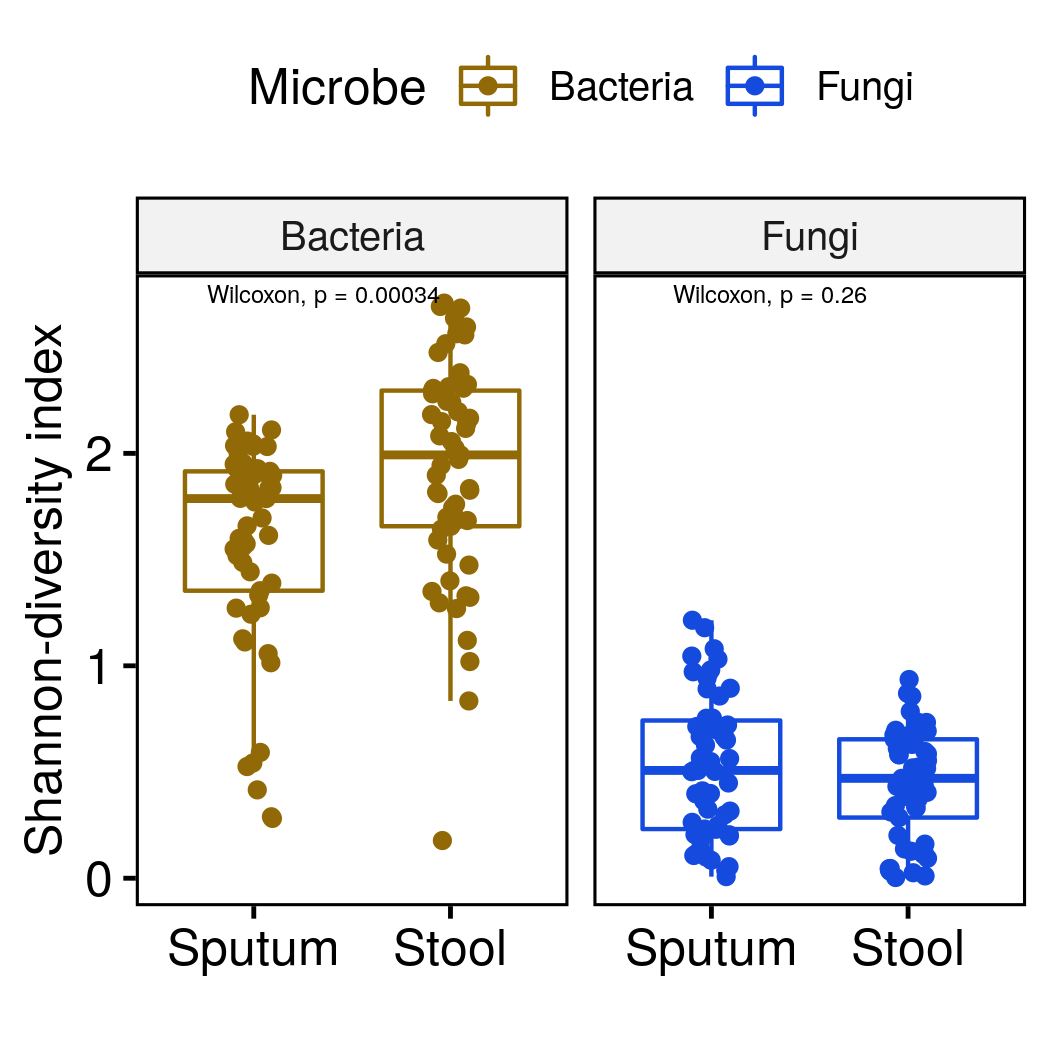
\includegraphics[width=0.5\textwidth]{image/diversity.png}
	\caption{A boxplot illustrating the difference in Shannon-diversity index of the Microbiome (Ochre) and Mycobiome (Blue) between the sputum (Lung) and stool (Gut) samples. Statistical significance of these differences were calculated using `wilcoxon test' and are indicated above as p-values.}
	\label{res2_fig1}
\end{figure}

\subsection{Co-occurrence analysis reveals lung – gut microbial (bacteria and fungi) interactions suggestive of a potential lung-gut axis.}
Assessment of interactions of microbes (bacteria and fungi) between the lung and gut was carried out using co-occurrence analysis. Co-occurrence analysis was performed using two methods 1)GBLM: captures complex linear interactions and 2) Spiec-easi: captures non-linear interactions but assumes sparsity, to derive microbial association networks. Microbial associations networks from both methods show cross-talk between the microbes of the lung and the gut, indicative of potential existence of the lung-gut axis [Figure\ref{res2_fig2}]. However, a greater number of inter-axis interactions is observed through the use of GBLM methods as compared to spiec-easi and this is partially due to the assumption of sparsity by spiec-easi. 

Integrative data-exploration of the microbiomes was performed using MOFA2. Roughly, MOFA2 works like a PCA to create factors which maximises the explained variance of the integrated microbiome. These learnt factors represent the driving sources of variation across the multiple input datasets, thus facilitating the identification of cellular states or disease subgroups. MOFA2 analysis using all four microbiomes (bacteria lung, bacteria gut, fungi lung and fungi gut) reveals a factor (Factor1) associated with exacerbations and Non-tuberculosis mycobacterial(NTM) infections [Figure\ref{res2_fig3}(c,d)]. Thus, establishing Factor1 as an important factor capable of capturing differences in exacerbation class and NTM\_ever(NTM infection ever) i.e., exacerbators (exacerbation = 1 and 2) and patients with no past history of NTM have a high median factor1 value compared to non-exacerbators (exacerbation=0) and patients with past history of NTM. Hence, following assessment of Factor1 in terms of contribution from individual microbiomes/datasets indicates the gut microbiome as the highest contributor as defined by the cumulative \% variance explained [Figure\ref{res2_fig3}(b)], possibly explainable by lung-gut axis hence lending further support to the existence of lung-gut axis. Moreover, upon assessment of the components of Factor1 (i.e., the microbes from the four microbiomes that make up factor1) we find four of the six overlapping microbes including \emph{Streptococcus, Saccharomyces, Candida} and \emph{Curvularia} have loadings $\geq 0.5\%$; implying that these microbes contribute $\geq 50\%$ towards factor1 from within their respective microbiomes.


\begin{figure}[h]
	\centering
	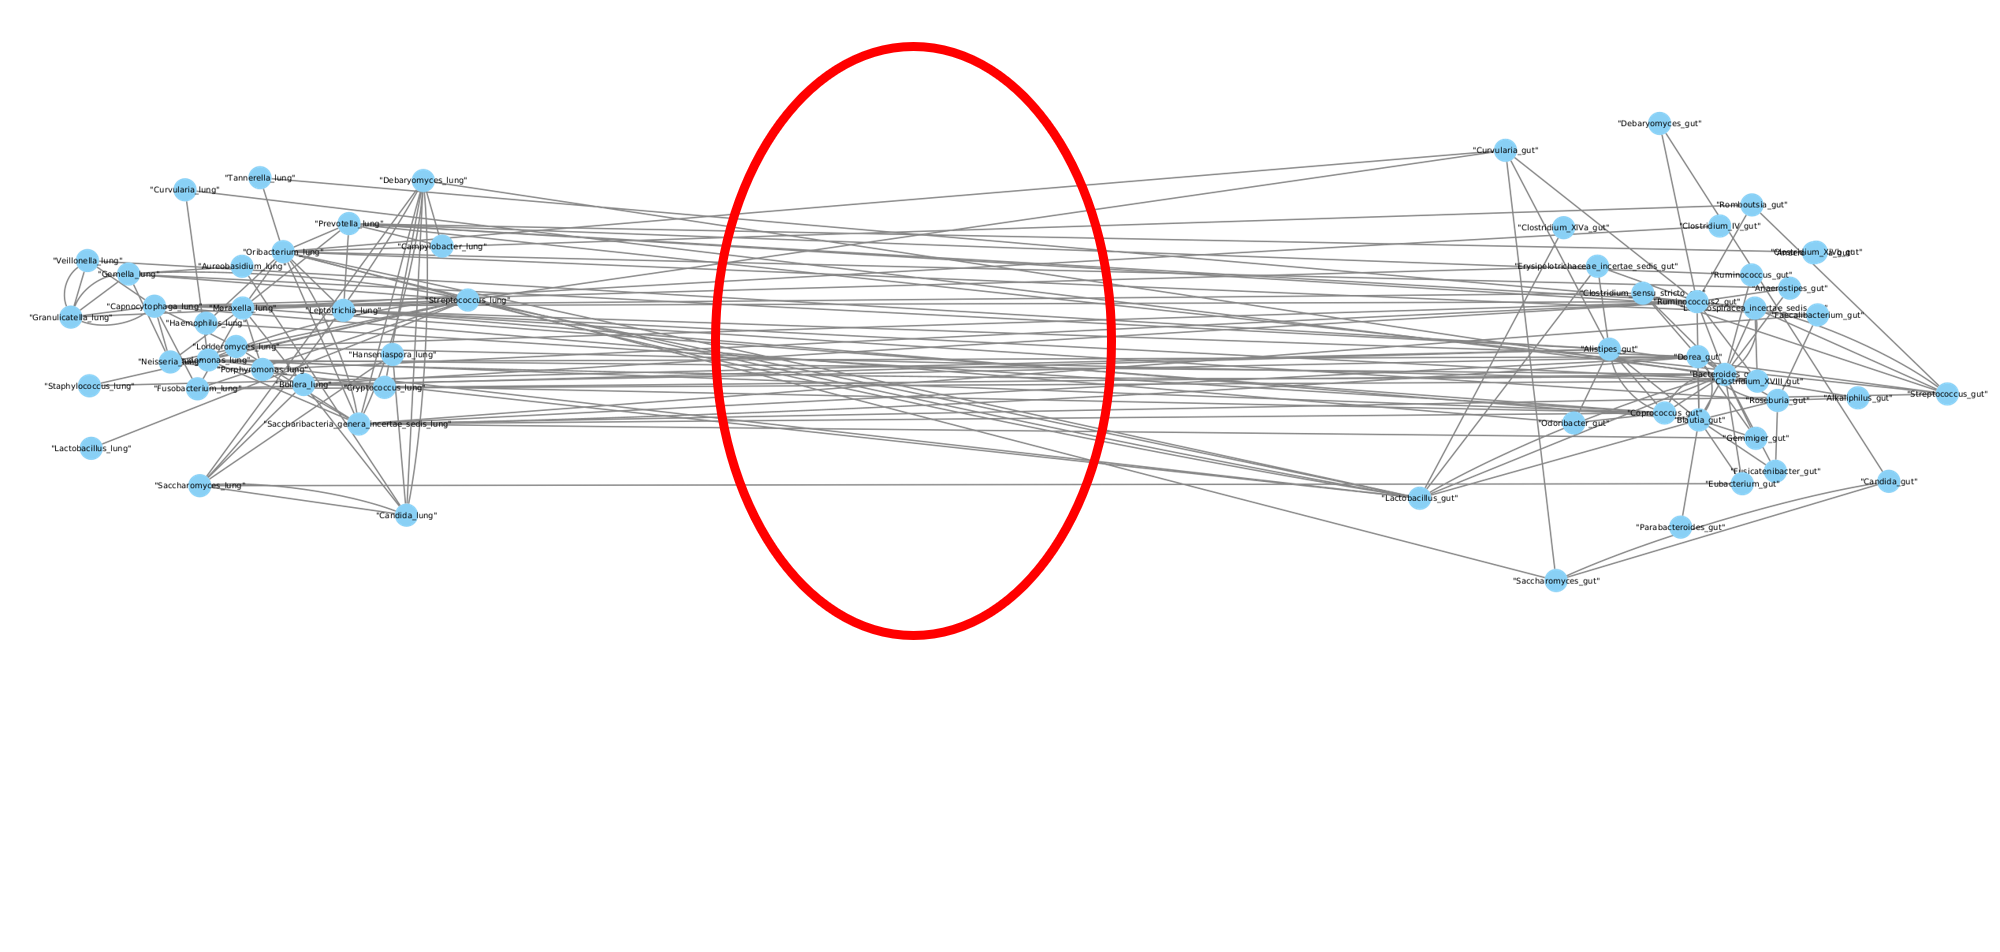
\includegraphics[width=\textwidth]{image/ch2-gblm-all.png} 
	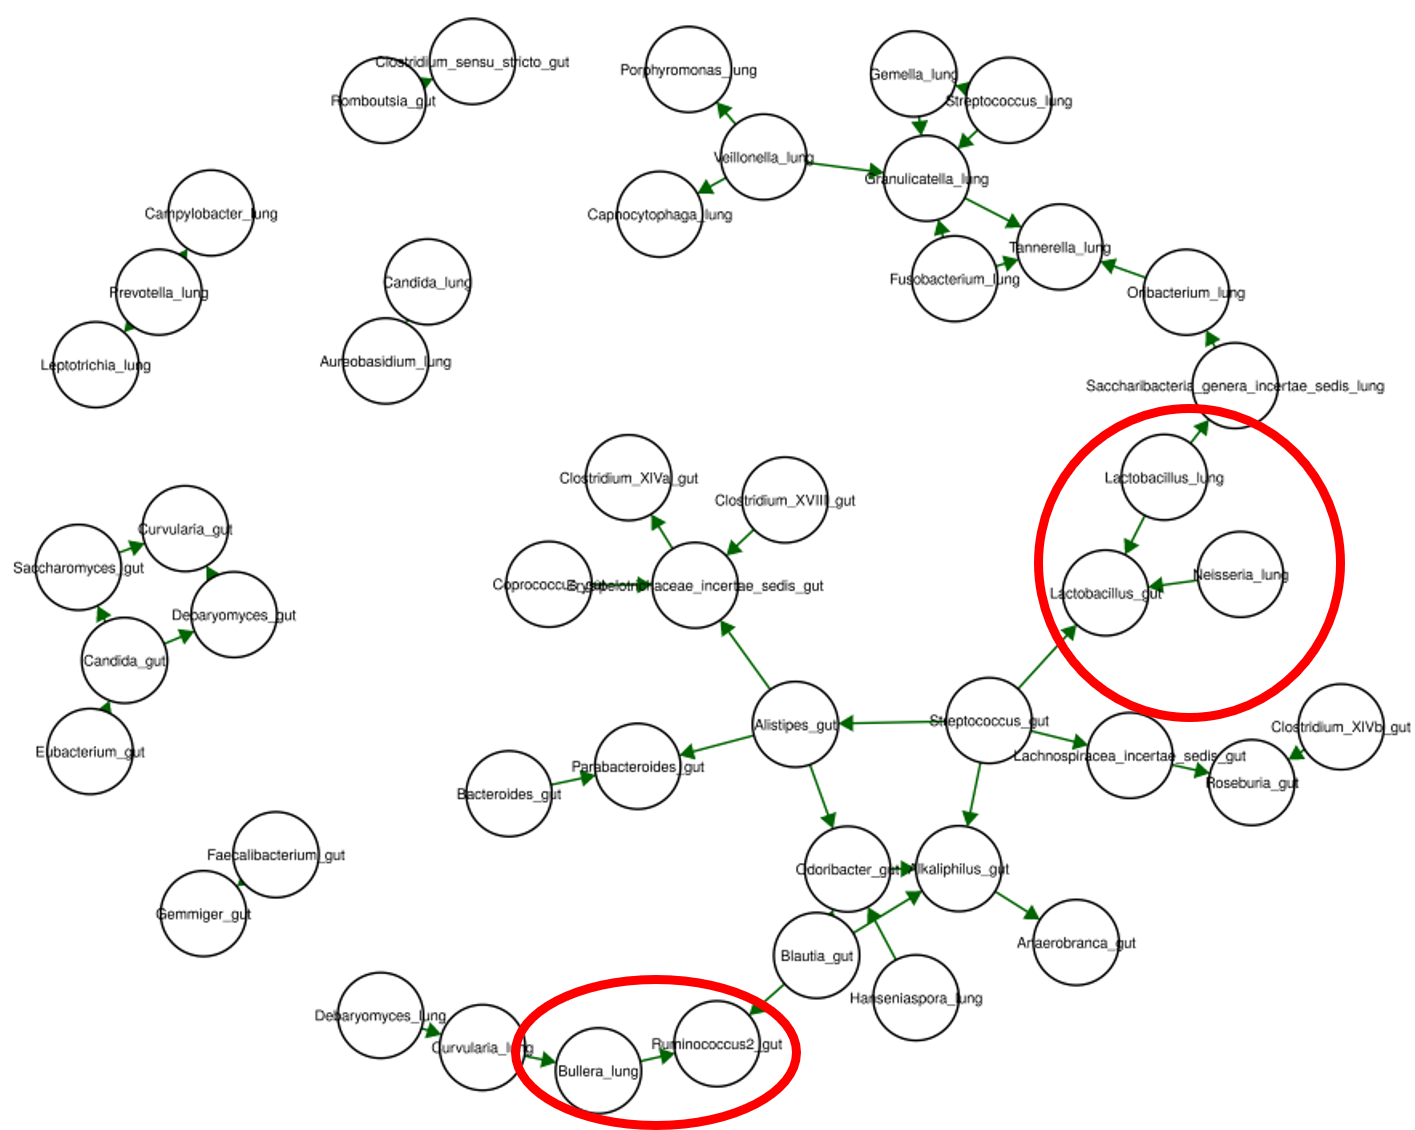
\includegraphics[width=0.6\textwidth]{image/ch2-se-all.png}
	\caption{Microbial association networks derived using co-occurrence analysis methods 1) GBLM(top) and 2)Spiec-easi(bottom). Nodes represents microbes including bacteria and fungi from both lung(left) and gut(right). Edges illustrate the association/interactions between the microbes derived using the respective methods. Highlighted red circle represents the interactions between the lung and gut microbiome.}
	\label{res2_fig2}
\end{figure}

\begin{figure}[h]
	\centering
	\subfloat[]{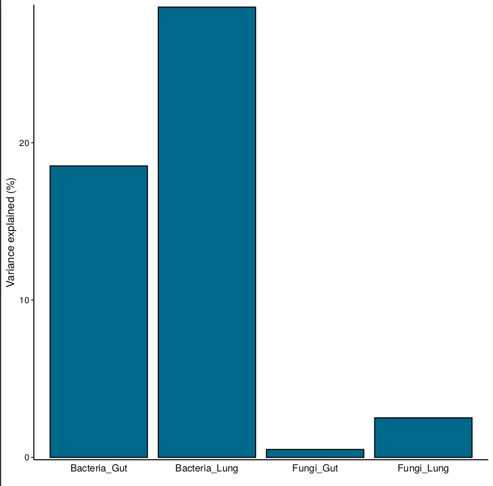
\includegraphics[width=0.4\textwidth]{image/ch2_bar_varex.png}}
	\subfloat[]{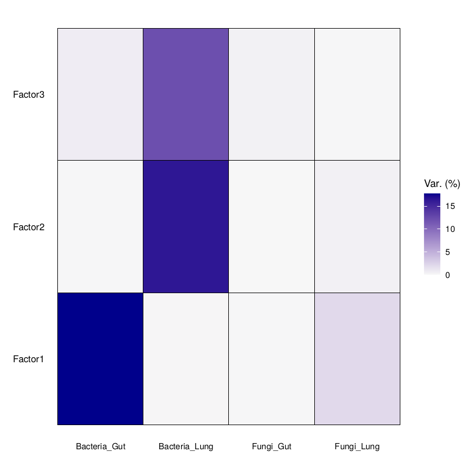
\includegraphics[width=0.4\textwidth]{image/ch2_heatmap_varex.png}}\\
	\subfloat[]{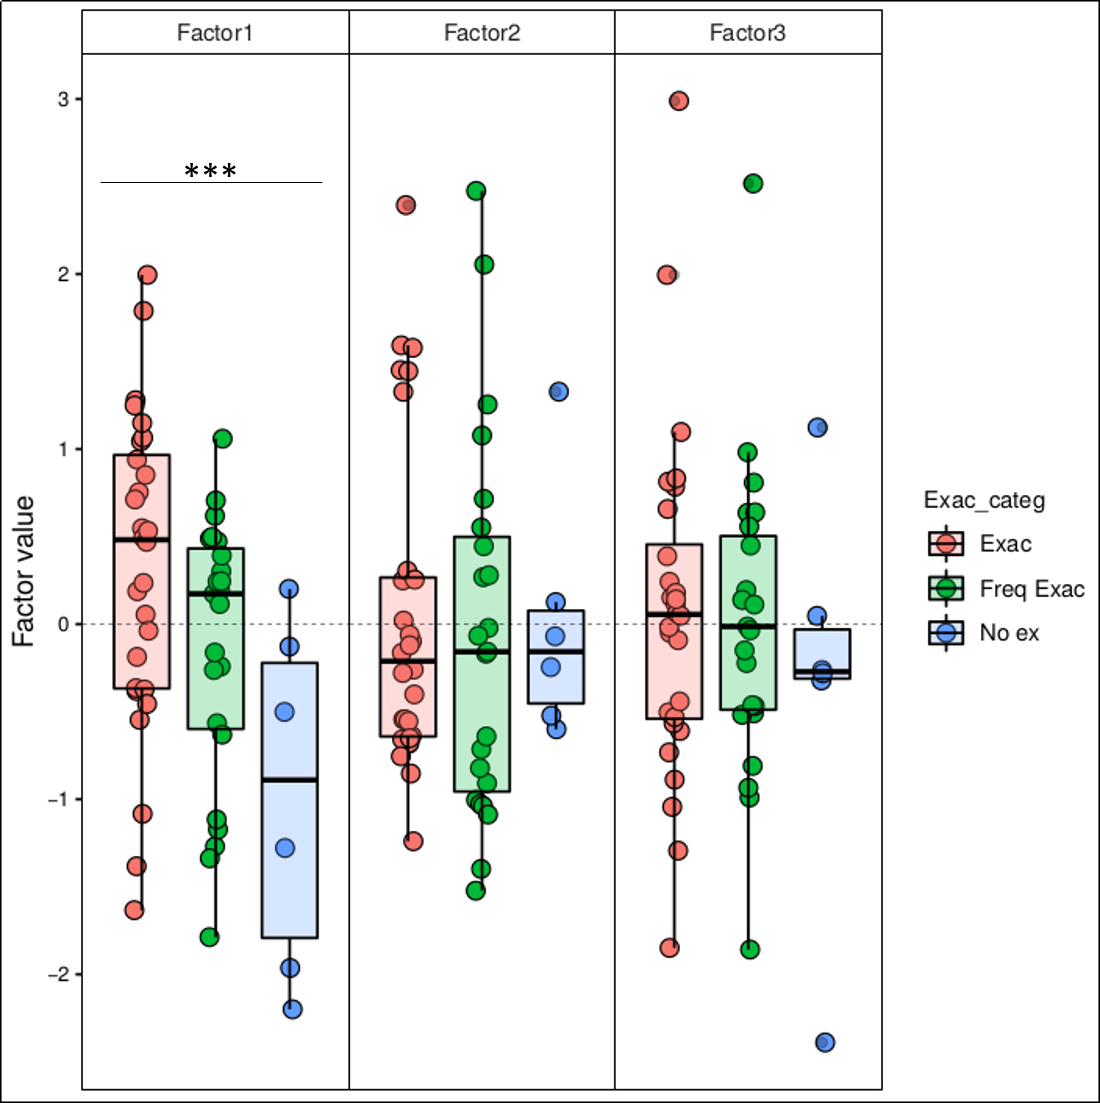
\includegraphics[width=0.4\textwidth]{image/ch2_mofa_exac.png}}
	\subfloat[]{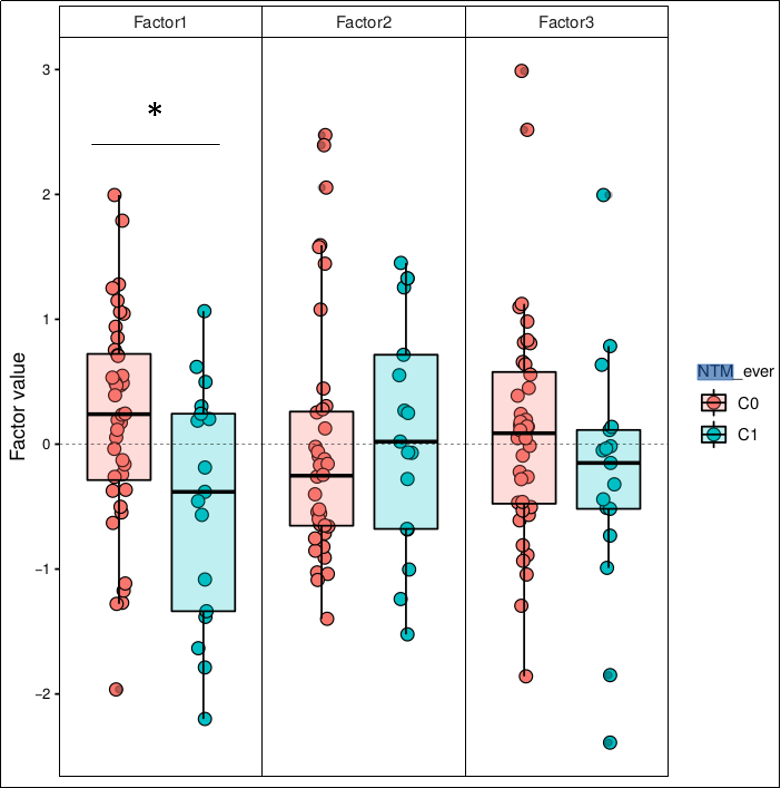
\includegraphics[width=0.4\textwidth]{image/ch2_mofa_NTM.png}}
	\caption{Integrative microbiome data analysis using MOFA2: (a) A bar chart representing the cumulative variance explained by each of the individual integrated biomes. (b) A heat-map illustrating the breakdown for variance explained of the individual biomes across the first three factors. Box plots illustrating the factor values of factors 1,2 and 3 across exacerbation category: `No ex' (Exacerbations = 0), `Exac' (Exacerbation = 1 to 2), `Freq Exac' (Exacerbation $\geq 3$) (c) and NTM\_ever (C0: Patient never had an NTM infection, C1: Patient had an NTM infection) groups (d).`*' illustrate the statistical significance of kruskal-wallis test in terms p-values; `*' p-value $<$ 0.05, `**' p-value $<$ 0.001,`***' p-value $<$ 0.0001}
	\label{res2_fig3}
\end{figure}

\subsection{Integrated microbiomes identifies a `high-risk' patient cluster}
Integration of microbiomes and mycobiomes from lung and gut using weighted SNF (wSNF) with k=9 was performed, followed by spectral clustering implemented to cluster the patients into two groups. Li \emph{et.al.} in their paper showed that integrating multiple views of the same patient/sample increases the power and compensates for smaller sample sizes\cite{Li2018}. Hence, clustering of the integrated microbiomes of these (n=57) patients is admissible. Cluster robustness was evaluated using a bootstrap approach and was found to be 79.15\%. Evaluation of the derived clusters across clinical attributes reveals patients belonging to cluster1 have a higher median risk of exacerbation, FACED score and Reiff score [Figure\ref{res2_fig4}] compared to cluster2. Differential abundance analysis illustrates significantly increased median clr abundace of \emph{Candia} in Gut ($1.97<3.23$) and \emph{Fusobacterium} in Lung ($1.71<2.90$), of high-risk patients (cluster1) compared to that of low-risk patients(cluster2). Furthermore, these microbes also contribute significantly to factor1 from the MOFA2 analysis. Evaluation of the loadings of \emph{Candia} Gut \emph{Fusobacterium} Lung reveal that have negative loadings and hence impact negatively the factor1 score. Figure\ref{res2_fig3}(c) shows that a lower median factor1 value corresponds to non-exacerbator and hence low-risk. Differential analysis reveal a higher abundance of these microbes in cluster2 compared to cluster1 and hence a lower factor1 value which implies a lower exacerbation as observed [Figure\ref{res2_fig4}(a)]. This further complements the integrative analysis and establishes its validity. MOFA2 analysis in confluence with differentially analysis provides explain-ability to the clusters derived based on wSNF analysis.
\begin{figure}[h]
	\centering
	\subfloat[]{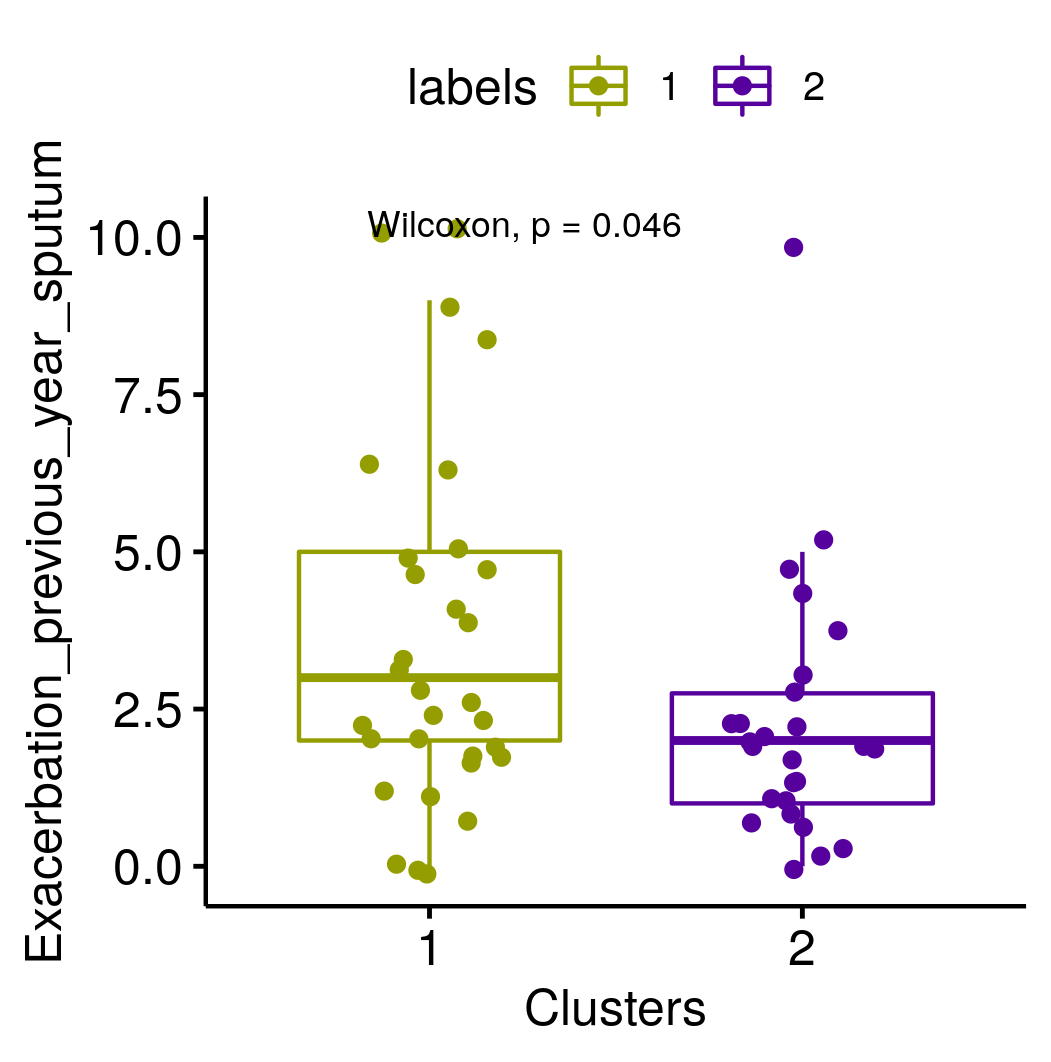
\includegraphics[width=0.3\textwidth]{image/Exacerbation_previous_year_sputum.png}}
	\subfloat[]{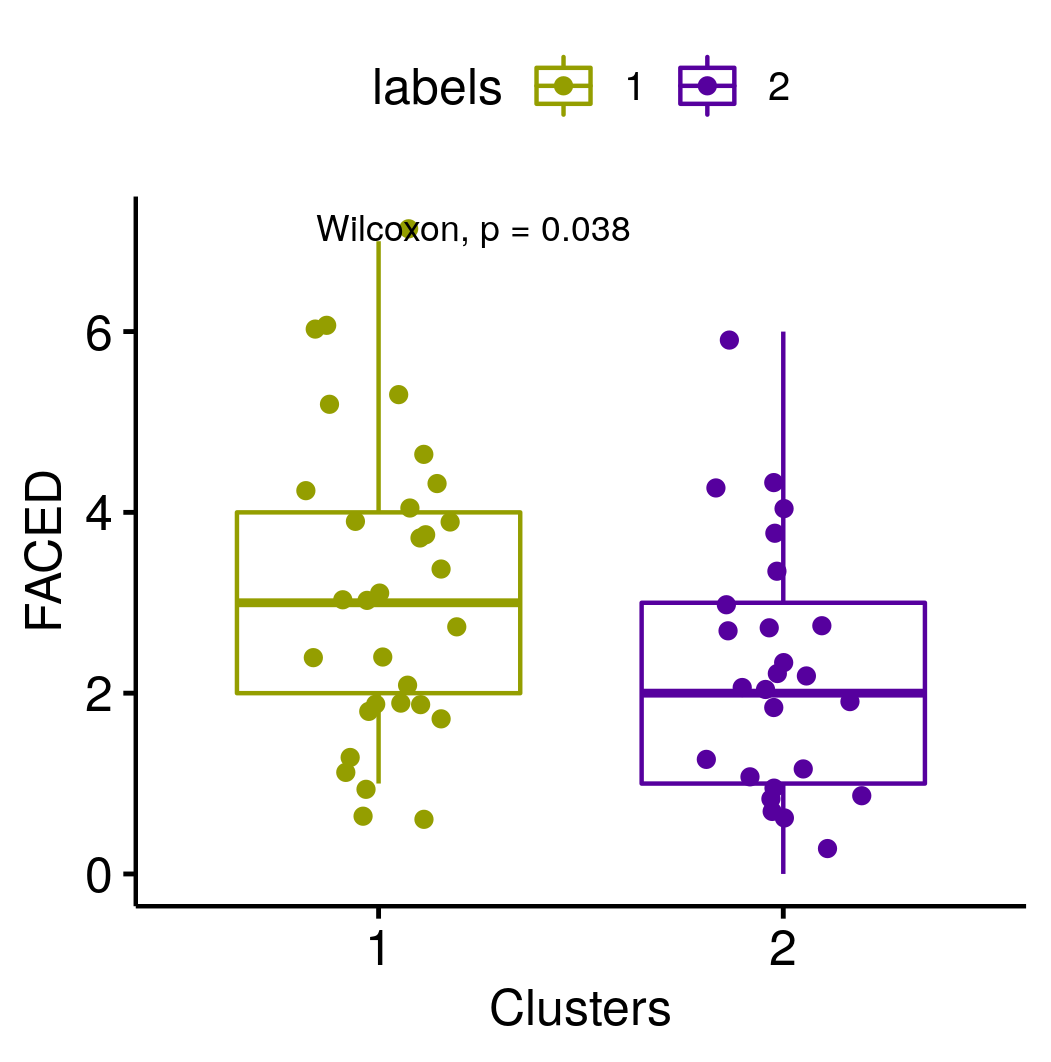
\includegraphics[width=0.3\textwidth]{image/FACED.png}}
	\subfloat[]{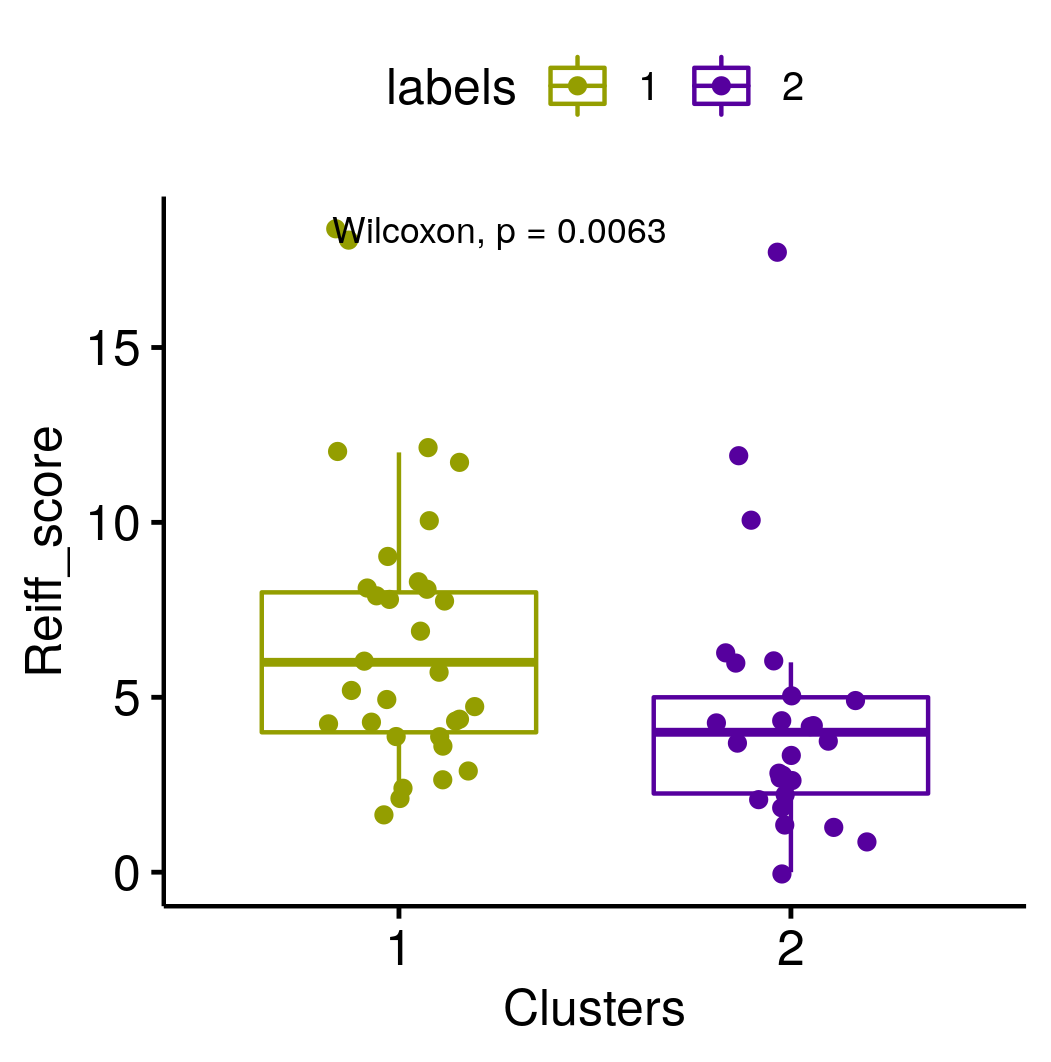
\includegraphics[width=0.3\textwidth]{image/Reiff_score.png}}
	\caption{Boxplots illustrating the differences in Exacerbation (a), FACED (b) and Reiff score (c) between high-risk cluster 1(yellow) and low-risk cluster 2(blue). Statistical significance of these differences were calculated using ‘wilcoxon test’ and are indicated above as p-values.}
	\label{res2_fig4}
\end{figure}

\subsection{Dysregulated lung-gut axis in high-risk patients}
Having shown the existence of lung-gut axis and identifying a sub-group of high-risk bronchiectasis patients using the integrative microbiomics; we next evaluated the changes in lung-gut axis across the two clusters. Microbes between the lung and gut can broadly interact in two ways: 1) Microbes can travel between the sites through mechanisms such as micro-aspiration and 2) Microbes can secrete secondary metabolites and other biomolecules through which they can interact. To assess the first mechanism, a linear correlation analysis between the clr transformed abundance of the overlapping microbes from the lung and gut was performed. \emph{Lactobacillus} lung was found to be significantly correlated with  \emph{Lactobacillus} gut in high-risk cluster 1 but not in cluster 2. However, the observed correlation of \emph{Lactobacillus} between the two sites may be due to confounding microbes. Therefore, a GBLM analysis was performed to assess the association of overlapping microbes between the two sites given all the other microbes. Interestingly, the correlation between \emph{Lactobacillus} lung and \emph{Lactobacillus} gut disappears. However, a new association between \emph{Streptococcus} lung and \emph{Streptococcus} gut is found in high-risk cluster 1 but not in low-risk patients; suggestive of movement of \emph{Streptococcus} between lung and gut in high-risk patients (probably due to dysregulation of the axis) [Figure\ref{res2_fig5}(a)]. Assessment of the second mechanism was performed by evaluating the inter-axis microbial interactions between clusters. This reveals an increased lung-gut microbial interaction in high-risk cluster(35\%) compared to low-risk cluster(29\%) [Figure\ref{res2_fig5}(b)]; further supplementing the dysregulation of this axis in high-risk patients.

\begin{figure}[h]
	\centering
	\subfloat[]{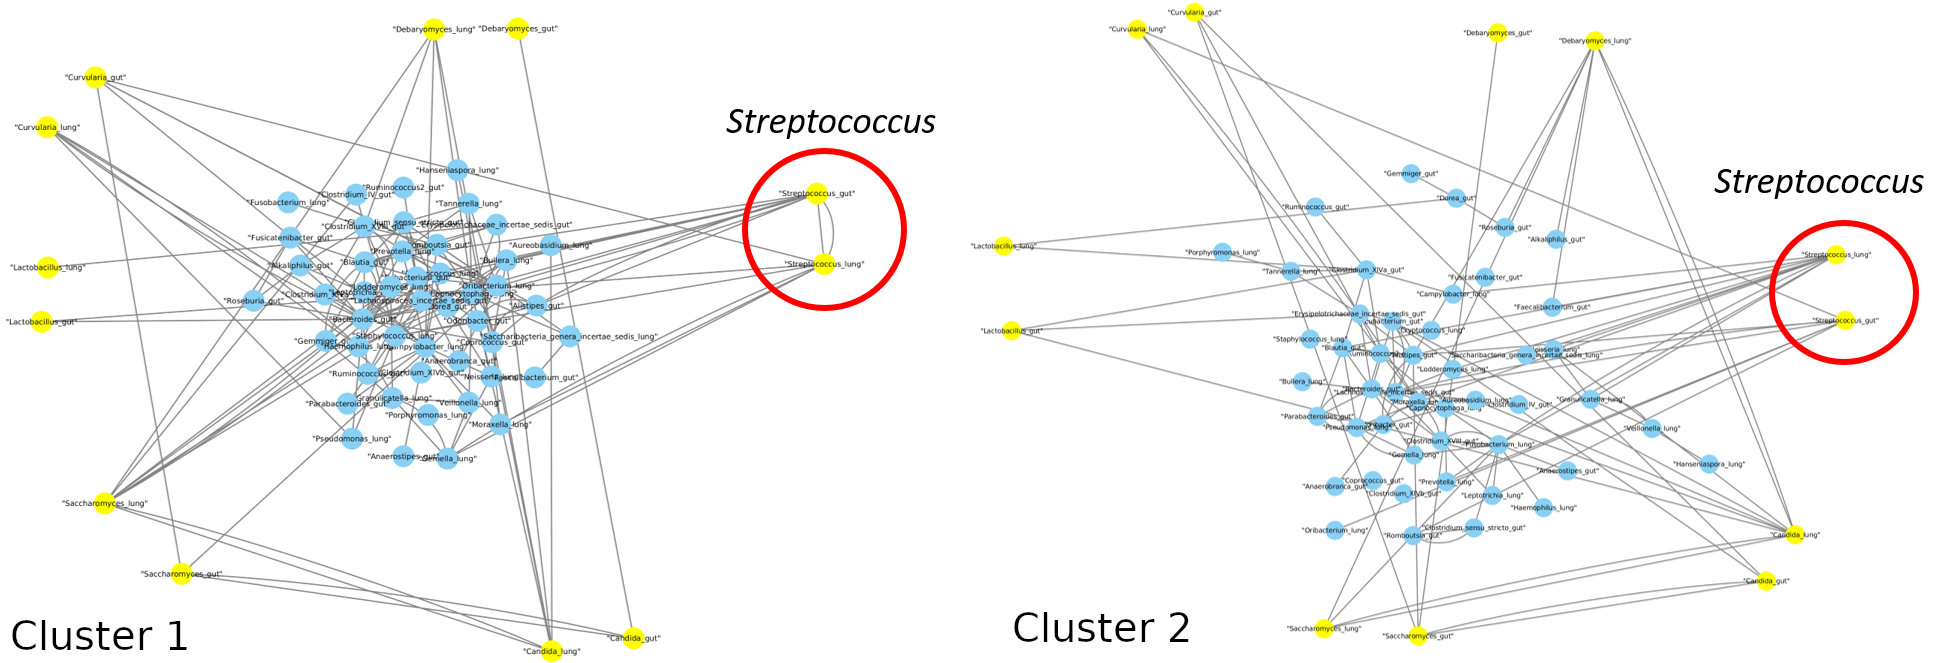
\includegraphics[width=\textwidth]{image/ch2_gblm_strep.png}}\\
	\subfloat[]{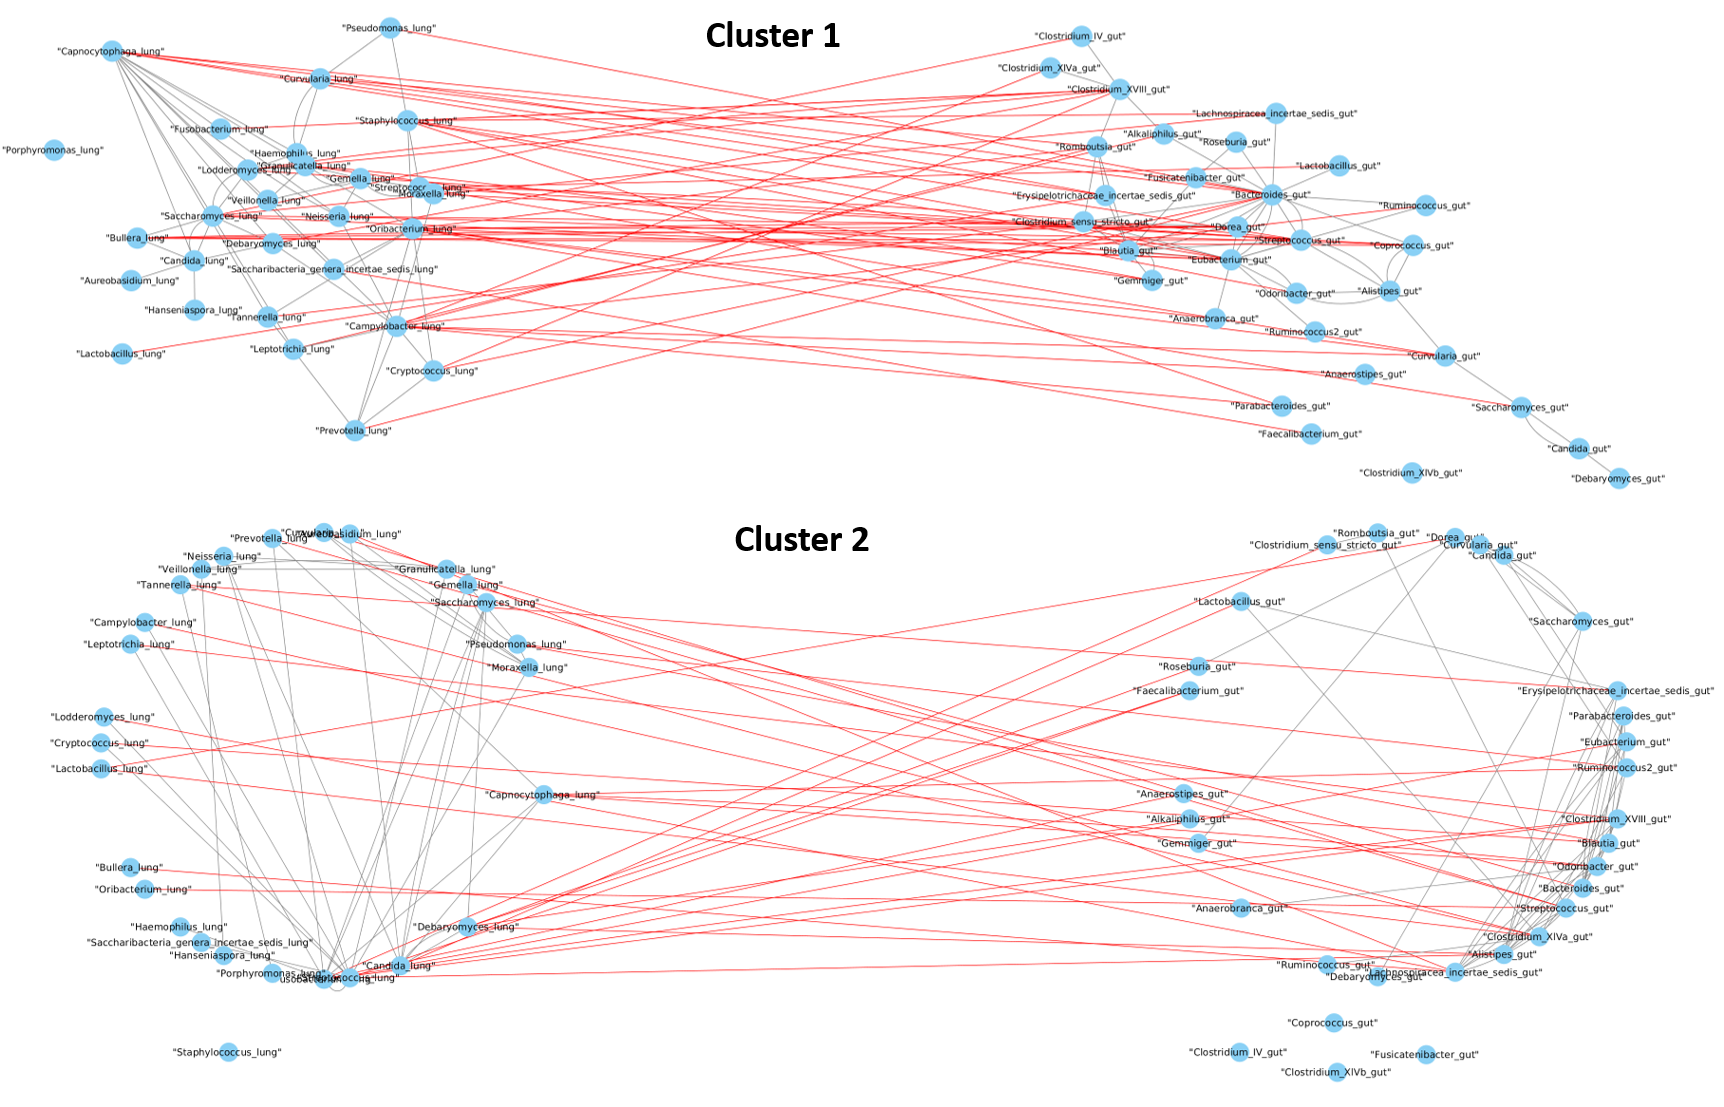
\includegraphics[width=\textwidth]{image/ch2_gblm_clusters.png}}
	\caption{Microbial co-occurrence network across the clusters, derived using GBLM with nodes as microbes (bacteria and fungi) from both lung and gut, and edges representing the significant (p-value$<$0.0001) interaction between nodes. (a) Overlapping microbes are highlighted as yellow nodes. (b) Inter lung-gut microbial interactions are highlighted as red edges.}
	\label{res2_fig5}
\end{figure}